\newpage
\section{Budowa sztucznej skóry}
\label{s_budowa}

\subsection{Otrzymany prototyp i stan badań}

Otrzymane w ramach pracy materiały związane z prototypem składały się z:
\begin{itemize}
    \item prototypu czujnika o rozmiarze $4x4$ pola i wymiarach $40x40 cm$ (rysunek \ref{f_otrzymany_prototyp}),
    \item układu elektronicznego obsługującego prototyp i komunikującego się z komputerem,
    \item wersji otwartej programu wgranego na mikrokontroler,
    \item oprogramowania w języku Python obrazującego odczyty napięcia ze sztucznej skóry ( rysunek \ref{f_otrzymany_apka}),
    \item dokumentacji zawierającej wykonane badania i opis budowy prototypu.
\end{itemize}

Otrzymany prototyp był zbudowany z dwóch fragmentów gumy typu NBR190 o wymiarach $40x40 cm$ i grubości $10 mm$ służących jako warstwy nośne, absorbujące uderzenia i rozkładające nacisk. Wewnątrz, na każdej z gum, zostały naklejone równolegle 4 paski taśmy miedzianej o szerokości $50 mm$ mające za zadanie przewodzić sygnały elektryczne. Taśma miedziana została naklejona na gumach w taki sposób, aby po ich złożeniu tworzyć matrycę przecięć o rozmiarze $4x4$. Do końcówek taśmy miedzianej z jednej strony zostały przylutowane przewody, które zostały dalej wyprowadzone na płytkę stykową. Pomiędzy warstwami gumy została umieszczona pojedyncza warstwa folii Velostat o wymiarach $30x30 cm$. Wszystkie elementy wewnętrzne zostały zabezpieczone przed przesuwaniem przez przyklejenie ich taśmą izolacyjną do powierzchni gumy. Obie warstwy gumy zostały ze sobą złączone trzema śrubami z użyciem szerokich podkładek, aby nie deformować nadmiernie gumy, oraz z użyciem nakrętek motylkowych, aby ułatwić późniejsze składanie i rozbieranie prototypu. Czwarty róg pozostał nieskręcony śrubą i~w~ten sposób umożliwiał w razie potrzeby na szybkie spojrzenie do wnętrza prototypu. Otrzymany prototyp wraz z~częścią elektroniczną znajduje się na rysunku \ref{f_otrzymany_prototyp} \cite{b_report_otrzymane}.

\begin{figure}[!h]
    \centering 
    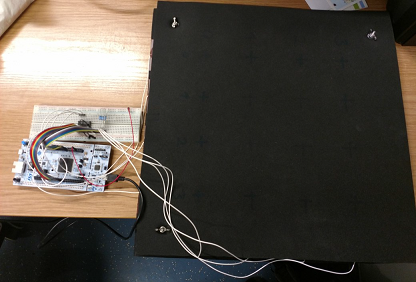
\includegraphics[width=0.95\linewidth]{img/otrzymane_prototyp.png}
    \caption{Otrzymany prototyp sztucznej skóry \cite{b_report_otrzymane}}
    \label{f_otrzymany_prototyp}
\end{figure}

Część sterująca prototypu została skonstruowana na płytce rozwojowej Nucleo-F767ZI. Pozostała część układu elektrycznego została wykonana na płytce stykowej i w głównej mierze składała się z drabinki Darlingtonowej ULN2003A. Drabinka ta odpowiadała za przełączanie pomiędzy odczytami poszczególnych wierszy czujnika. Kolumny czujnika były podłączone bezpośrednio do mikrokontrolera STM32F767ZIT6U, do wbudowanych w~mikrokontroler przetworników analogowo-cyfrowych \cite{b_report_otrzymane}.

Program zapisany na mikrokontrolerze był bardzo prosty, a jego jedynym zadaniem było ciągłe przełączanie poszczególnych wierszy i kolumn oraz odczyt wartości dostępnych na pinach przetwornika analogowo-cyfrowego z częstotliwością około $\sim10 Hz$. Program, od~razu po wykonaniu odczytu, konwertował go ze stanu surowego na wartość odczytanego napięcia i taki odczyt wysyłał do komputera. Sygnał wysyłany był przez mikrokontroler interfejsem UART, a układ programatora ,instalowany fabrycznie na wszystkich płytkach z~serii Nucleo, przesyłał te dane dalej do komputera za pośrednictwem interfejsu USB \cite{b_report_otrzymane}.

Po stronie komputera zostało napisane oprogramowanie pozwalające na odczytywanie wiadomości wysyłanych przez mikrokontroler. Oprogramowanie napisano w Pythonie z~użyciem biblioteki PyQT i zaimplementowano mu prosty oraz intuicyjny interfejs. 
Wykonana aplikacja komputerowa przedstawiona jest na rysunku \ref{f_otrzymany_apka}.
Po lewej stronie znajduje się wizualizacja przyłożonej siły, gdzie każdy kwadrat odpowiada jednemu polu czujnika. Im większa siła została przyłożona do danego pola, tym jaśniejsze staje się pole na ekranie. Po prawej stronie interfejsu znajduje się natomiast wykres odczytanych wartości z~ostatnich kilkudziesięciu sekund z~jednego pola. Wykres przedstawia napięcie na polu sztucznej skóry w~zależności od czasu i~pozwala nie tylko odczytać dokładne wartości wykonanego pomiaru, ale~przede wszystkim jak ten pomiar się zmieniał.
Nad~wykresem znajdują się rozwijane listy pozwalające wybrać, pomiary którego czujnika chcemy aktualnie obserwować  \cite{b_report_otrzymane}.

\begin{figure}[!h]
    \centering 
    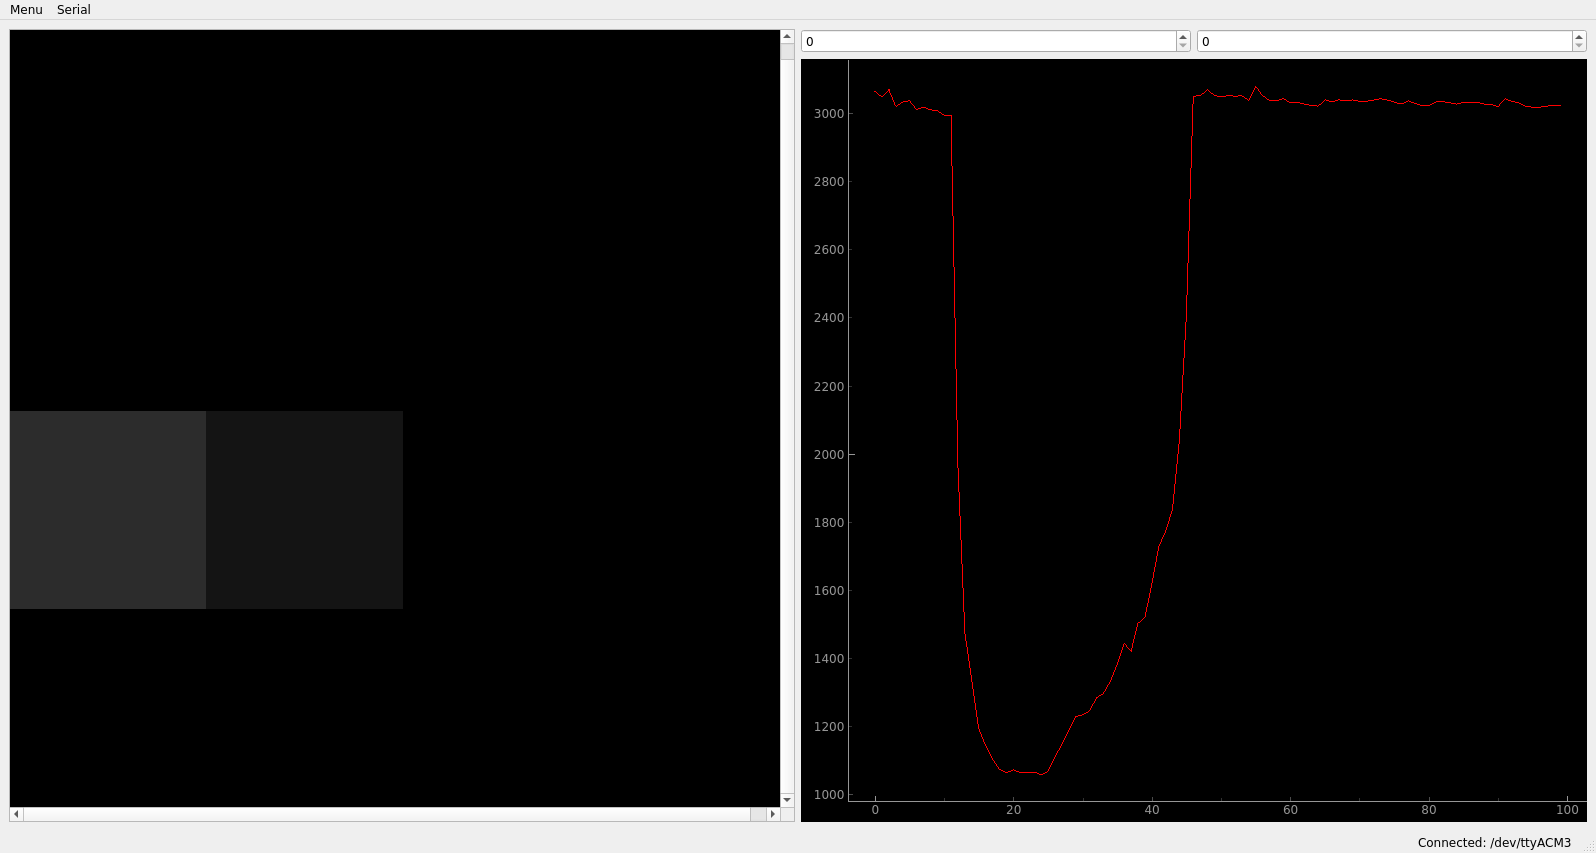
\includegraphics[width=0.95\linewidth]{img/otrzymane_apka.png}
    \caption{Otrzymana aplikacja odczytująca pomiary ze sztucznej skóry \cite{b_report_otrzymane}}
    \label{f_otrzymany_apka}
\end{figure}

Badania wykonane nad opisanym powyżej prototypem przebiegały głównie przed budową samego prototypu, a przedstawiony prototyp był ich zwieńczeniem. Prowadzone badania dotyczyły głównie wybrania odpowiednich rozwiązań i materiałów do budowy prototypu. Został wykonany przegląd literatury, którego efektem było ustalenie takiej budowy sztucznej skóry. Zostały ustalone założenia projektu oraz przystąpiono do wyboru materiałów. Jako materiał o zmiennej rezystancji została wybrana folia Velostat, a warstwy przewodzące folia miedziana. Aby dokonać wyboru najlepszego materiału nośnego zostały wykonane badania wielu (jedenastu) różnych rodzajów materiałów. Testowane one były pod kątem przewodności elektrycznej, trwałej odkształcalności i pochłanialności energii. Ostatecznie, jako materiał najlepiej spełniający postawione kryteria, wybrana została guma NBR190. Zwieńczeniem badań był opisywany wcześniej prototyp, na którym nie zostały wykonane żadne szczegółowe testy. Zostało tylko sprawdzone, czy rozwiązanie w ogólnym zakresie działa tak, jak było to przewidywane. Te nieskomplikowane testy przeszły pozytywnie \cite{b_report_otrzymane}.

Bazując na przekazanym prototypie zostały wyznaczone wszystkie obszary, w~których należy przeprowadzić dalsze prace. Zostały wyznaczone 4 główne warstwy: mechaniczna, elektroniczna, komunikacyjna i programowa. Dokonane wybory wraz z uzasadnieniem zostały przedstawione w rozdziałach: \ref{ss_budowa_mech}~-~warstwa mechaniczna (czujnik), \ref{ss_integracja_budowa}~-~warstwa mechaniczna (mocowanie do robota), \ref{ss_budowa_ele}~-~warstwa elektroniczna, \ref{ss_budowa_kom}~-~warstwa komunikacyjna, \ref{ss_budowa_prog}~-~warstwa programowa (część sterownika), \ref{ss_integracja_Python} oraz \ref{ss_integracja_algorytm}~-~warstwa programowa (część węzła w systemie ROS).
Schemat projektowanej sztucznej skóry, wraz z~wyszczególnieniem zakresów pracy przy poszczególnych warstwach został przedstawiony na rysunku~\ref{f_art_skin_system}.

\begin{figure}[!h]
    \centering 
    \includegraphics[width=0.95\linewidth]{img/art_skin_system.pdf}
    \caption{Schemat systemu sztucznej skóry wraz z wyszczególnionymi warstwami, przy których prowadzono prace}
    \label{f_art_skin_system}
\end{figure}

\subsection{Warstwa mechaniczna}
\label{ss_budowa_mech}

Część mechaniczna jest pierwszym elementem widocznym po spojrzeniu na sztuczną skórę. Jednak poza przystępnym wyglądem musi ona spełniać dużo bardziej podstawowe funkcje części mechanicznych. Przede wszystkim jest to szkielet całej konstrukcji, który trzyma całość w skupionej postaci oraz zapobiega przemieszczaniu się elementów czujnika. Jest ona także odpowiedzialna za ochronę przed uszkodzeniami pochodzącymi ze środowiska zewnętrznego. Bazując na tym spisana została lista założeń, które projektowana część mechaniczna musiała spełniać:
\begin{itemize}
    \item podatność i odporność mechaniczna - czujnik powinien móc się ugiąć oraz pochłonąć energię uderzenia, aby ochronić robota i otoczenie przed uszkodzeniem,
    \item możliwość stosowania na nierównych powierzchniach i na krzywiznach obudowy robota,
    \item niska masa, biorąc pod uwagę docelowe duże rozmiary czujnika,
    \item uniwersalność i skalowalność czujnika - możliwość stosowania w różnych konfiguracjach na różnych robotach.
\end{itemize}

Większość postawionych założeń dotyczących części mechanicznych jest spełniana przez użytą gumę mikroporowatą. Dlatego też to guma była dobierana do założeń projektowych tak, aby je spełniała.

Mechanicznie, budowa mojej wersji czujnika nie różniła się w dużej mierze od prototypu, który został mi przekazany jako podstawa prac. Czujnik również został zbudowany z~pięciu podstawowych warstw: mechanicznej zewnętrznej (guma), przewodzącej zewnętrznej (poziome paski folii miedzianej), folii Velostat, przewodzącej wewnętrznej (pionowe paski folii miedzianej) oraz mechanicznej wewnętrznej (guma). Jedynymi modyfikacjami wykonanymi w ramach pracy było dobranie doświadczalnie odpowiednich grubości gumy oraz rozbudowanie wewnętrznej warstwy nośnej czujnika o sztywny szkielet, będący łącznikiem pomiędzy giętkim czujnikiem, a obudową robota \cite{b_report_otrzymane}. Wykorzystana w~czujniku kolejność warstw została zobrazowana na rysunku \ref{f_otrzymany_budowa}.

\begin{figure}[!h]
    \centering 
    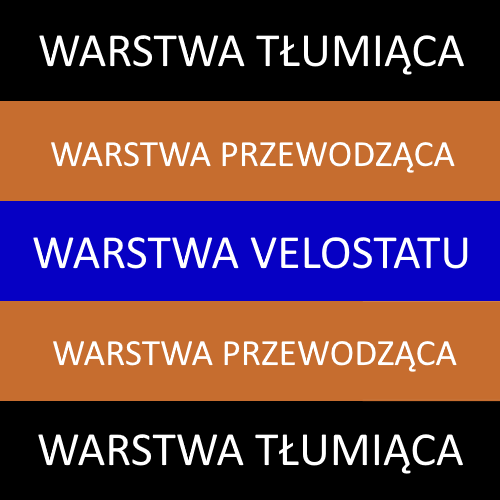
\includegraphics[width=0.5\linewidth]{img/otrzymane_budowa.png}
    \caption{Przekrój budowy sztucznej skóry \cite{b_report_otrzymane}}
    \label{f_otrzymany_budowa}
\end{figure}

Aby utrzymać wszystkie warstwy złączone ze sobą nie zostały wykorzystane śruby, jak~w~poprzednim modelu, ponieważ one są bardzo kłopotliwe i nie zapewniają odpowiedniego zabezpieczenia, zarówno robota, jak i otoczenia. Jako materiał łączący warstwy ze sobą zostały użyte różnego rodzaju taśmy (montażowe, izolacyjne, dwustronne). Zapewniają one praktycznie niewidoczne połączenie pomiędzy warstwami i~nie wystają poza obręb zewnętrznej gumy. Najważniejszą ich zaletą jest jednak fakt, że nie wywierają one istotnych naprężeń w~warstwie gumy, co znacznie poprawia wyniki w~porównaniu z~wersją, gdzie czujnik jest skręcony śrubami.

\subsection{Warstwa elektroniczna}
\label{ss_budowa_ele}

Sterownik sztucznej skóry jest jedną z pierwszych warstw (zaraz za warstwą fizyczną czujnika), która odpowiada za poprawne działanie całego systemu. Informacje przez niego odczytywane są przesyłane bezpośrednio do systemu sterowania robotem. Z tego powodu jest to bardzo ważne, aby ta część działała prawidłowo i niezawodnie. Potencjalne złe działanie sterownika sztucznej skóry może skutkować wysyłaniem do komputera całkowicie nieprawdziwych informacji, a co za tym idzie działanie całego robota będzie nieprzewidywalne, wręcz niebezpieczne.

Warto zauważyć, że w tym projekcie jest to ostatnie miejsce, gdzie sygnał występuje jeszcze w formie analogowej - odczyty z poszczególnych pól czujnika są analogowe. Dane wysyłane z czujnika są już natomiast wysyłane przez magistralę USB w formie cyfrowej. Z~tego powodu ważne jest, aby na tym etapie wyeliminować możliwie dużo zakłóceń, które są przyczyną występowania błędów na sygnałach analogowych.

Zastosowany do tego zadania sterownik musi spełniać szereg różnych zadań, spośród których najważniejsze są:
\begin{itemize}
    \item obsługa wszystkich pól sztucznej skóry, poprzez odpowiednie doprowadzenie zasilania i odczyt wartości nacisku na pole,
    \item zapewnienie ciągłości i poprawności wykonywanych pomiarów,
    \item agregowanie pomiarów ze wszystkich pól i przesyłanie ich do jednostki sterującej w~formie łatwiejszej do dalszej obsługi,
    \item automatyczny reset w przypadku błędów krytycznych lub zawieszenia się systemu,
    \item szybka i stabilna komunikacja z komputerem nadrzędnym z wykorzystaniem standardowego łącza komunikacyjnego,
    \item prawidłowe działanie bez konieczności dołączania dodatkowego źródła zasilania (baterie, akumulatory) - zasilanie z~komputera nadrzędnego,
    \item możliwość częściowej rekonfiguracji systemu bez konieczności zmiany programu mikrokontrolera.
\end{itemize}

Wymienione powyżej zadania zostały sprecyzowane przed przystąpieniem do prac i~pozwoliły na~dobór odpowiednich środków do wyznaczonych celów. Wykonany w~celu obsługi sztucznej skóry układ, spełniający przedstawione założenia, przedstawiony jest na rysunku \ref{f_elektronika_moja}.

\begin{figure}[!h]
    \centering 
    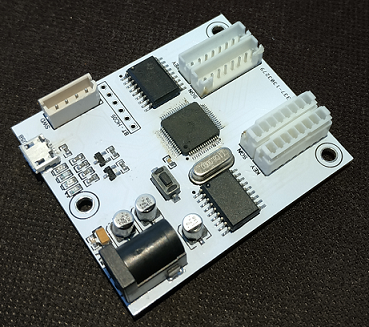
\includegraphics[width=0.5\linewidth]{img/elektronika_moja.png}
    \caption{Zaprojektowany układ elektroniczny do obsługi sztucznej skóry}
    \label{f_elektronika_moja}
\end{figure}

Do poprawnego działania sterownika potrzebny jest mikrokontroler. Wybór padł na opisywany już wcześniej w tej pracy STM32, a~dokładniej STM32F103RB. Mikrokontroler ten jest bardzo prosty, posiada niewielką ilość pamięci Flash i podstawowe peryferia. Pośród posiadanych przez niego peryferiów znajdują się kluczowe dla tego projektu przetworniki analogowo-cyfrowe, które pozwalają na bezpośrednie odczytywanie wartości napięcia na odpowiednim wejściu mikrokontrolera. Przetworniki analogowo-cyfrowe zostały w taki sposób, aby bezpośrednio mierzyć napięcie odkładające się na polu czujnika sztucznej skóry. Schemat podłączenia przetworników analogowych do sztucznej skóry widoczny jest na rysunku \ref{f_elektronika_schemat}. Pozostałe wykorzystywane w tym projekcie peryferia mikrokontrolera nie miały dużego znaczenia przy wyborze modelu, ponieważ znajdują się one w prawie każdym dostępnym na rynku mikrokontrolerze. Mimo wszystko przy wyborze największe znaczenia miała moja wcześniejsza znajomość z tym konkretnym modelem \cite{b_site_F103RB}.

\begin{figure}[!h]
    \centering 
    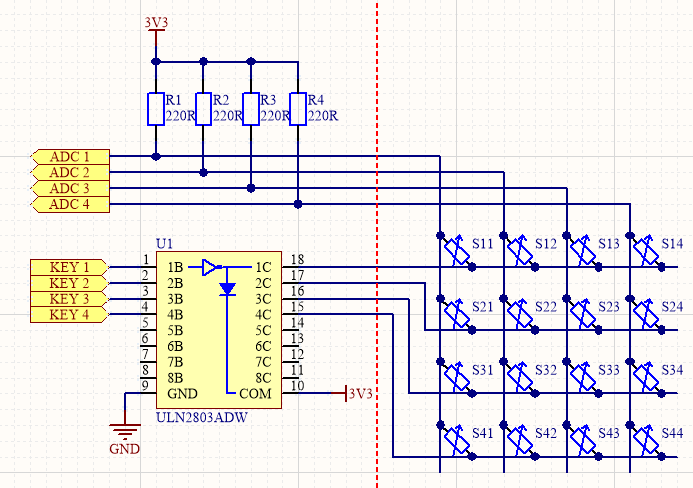
\includegraphics[width=0.95\linewidth]{img/elektronika_schemat.png}
    \caption{Schemat elektroniczny sposobu działania sztucznej skóry}
    \label{f_elektronika_schemat}
\end{figure}

Na schemacie połączeniowym, przedstawionym na rysunku \ref{f_elektronika_schemat}, widoczny jest także układ ULN2803ADW. Układ ten jest drabinką Darlingtonową (drabinką tranzystorów bipolarnych połączonych w~układ Darlingtona) i pełni funkcję klucza zwierającego poziome wiersze czujnika do masy. W~praktyce nie zwiera tych linii do masy tylko do wartości około $0.75 V$, co było mocno widoczne na możliwym do uzyskania zakresie pomiarów, który z~tego powodu był dużo mniejszy \cite{b_site_ULN2803}. Do układu dochodzi sygnał kluczujący, który steruje aktualnie wybranym wierszem, przy czym w danej chwili tylko jeden z nich może być wybrany. W przeciwnym wypadku pomiary będą błędne.

Konstrukcję elektroniczną uzupełniają dość standardowe elementy jak przycisk resetu mikrokontrolera, diody LED sygnalizujące stan pracy urządzenia, stabilizatory ustalające napięcie pracy układu, czy też zabezpieczenia źródła zasilania. Jeśli chodzi o zabezpieczenia, to jako wystarczające zabezpieczenia dla tego projektu uznane zostały: zabezpieczenie przeciwzwarciowe, nadnapięciowe i przed odwróconą polaryzacją źródła zasilania. Zabezpieczenia te zostały zostały dodane w razie potrzeby, ale z racji specyfiki pracy i zasilania przez port USB nie powinny one nigdy zostać w pełni wykorzystane.


% \subsubsection{Oprogramowanie mikrokontrolera}
\subsection{Warstwa programowa}
\label{ss_budowa_prog}

Oprogramowanie jest zwieńczeniem pracy nad sterownikiem. Zespala ono wszystkie spełniane funkcje oraz sprawia, że całość zaczyna spełniać swoje zadanie. Napisany program spełnia wymagania stawiane mu przez pozostałe elementy systemu oraz prawidłowo odczytuje, przetwarza i~interpretuje dane. Zawiera też kilka usprawnień względem kodu przekazanego wraz z prototypem. Program zawiera też w~sobie kilka podstawowych zabezpieczeń. Jednym z~nich jest zabezpieczenie watchdog przed utknięciem w~pętli lub zatrzymaniem działania. 

Główna część programu, zajmująca się przetwarzaniem wyników, pracuje w przerwaniu inicjowanym przez licznik. Część ta jest wywoływana przez program dokładnie z~częstotliwością $10 Hz$. Program w tym momencie wykonuje odczyty napięcia ze~wszystkich zapisanych w~konfiguracji czujników. Aby proces ten przebiegał szybko i~sprawnie przetworniki analogowo-cyfrowe zostały skonfigurowane we współpracy z DMA (direct memory access), który pozwala na przesyłanie danych z~peryferiów do pamięci bez wykorzystania procesora. Zestaw ten znacznie przyspiesza pomiary i~pozwala na~ich wykonywanie w~czasie kiedy procesor przetwarza dane z poprzedniego pomiaru. Po~wykonaniu wszystkich pomiarów dane są obliczane według opisanego dalej algorytmu, a~otrzymany wynik jest wysyłany do komputera.


\subsubsection{Opracowanie algorytmu obliczającego nacisk na wszystkie pola}
\label{sss_budowa_opracowanie_algorytmu}

Algorytm obliczający siłę i kierunek nacisku został napisany tak, aby agregować odczyty ze wszystkich pól czujnika i~przesłać je dalej w prostszej formie. Algorytm zakłada, że~każde pole czujnika jest umiejscowione na robocie i można opisać jego położenie za~pomocą odległości od środka robota i kierunkiem (kątem od środka osi robota). Zależność ta może być przestawiona jako wektory w dwuwymiarowym układzie współrzędnych biegunowych.

Obliczanie końcowego wektora siły odbywa się przez dodawanie do siebie wektorów z kolejnych pól czujnika. Po dodaniu wszystkich wektorów otrzymywany jest wektor wyjściowy siły nacisku i kierunku, który wysyłany jest później do jednostki nadrzędnej. W~ten sposób przesyłana dalej jest tylko kluczowa dla robota część informacji.

Obliczanie kolejnych wektorów siły jest wykonywane za pomocą opisanego algorytmu powtarzanego dla wszystkich pól:
\begin{align}
    F_x & = F_0 * cos(\alpha_0) + F_i * cos(\alpha_i) \\
    F_y & = F_0 * sin(\alpha_0) + F_i * sin(\alpha_i) \\
    F_0 & = \sqrt{F_x^2+F_y^2} \\
    \alpha_0 & = atan2(F_y,F_x)
\end{align}

We wzorze tym $F_i$ jest wartością siły odczytywanej z każdego kolejnego, $i$-tego pola sztucznej skóry. Analogicznie $\alpha_i$ jest wartością kąta kolejnych, $i$-tych pól sztucznej skóry. Zmienna $F_0$ jest skumulowaną wartością siły ze wszystkich kolejnych odczytanych pól sztucznej skóry, aż do $i$-tego pola. Podobnie $\alpha_0$ jest wynikową wartością kąta obliczonej siły $F_0$. Wartości $F_x$ i $F_y$ są chwilowymi przekształceniami siły nacisku oraz jej kąta z układu współrzędnych biegunowych na ich odpowiedniki w układzie kartezjańskim. Otrzymywane są w ten sposób wektory siły nacisku na robota w osiach $x$ i $y$. Przekształcenie wartości siły nacisku na układ kartezjański pozwala kumulować wektory siły odczytywane z kolejnych pól czujnika przez ich sumowanie.

Należy też zauważyć, że siła nacisku $F_i$ w powyższym równaniu obliczana jest bezpośrednio na podstawie odczytów z danego pola czujnika i jest obliczana na podstawie wyznaczonej eksperymentalnie hiperboli aproksymującej czujnik (wyznaczanie hiperboli zostało opisane w rozdziale \ref{ss_badanie_hiperbola}). Siła nacisku $F_i$ jest również na tym etapie dodatkowo dzielona przez odległość od środka robota, aby zmniejszyć wpływ skrajnie zewnętrznych pól czujnika i wzmocnić te bliżej środka robota (lub bardziej strategiczne). Wzmacnianie i~osłabianie wartości siły pochodzącej z czujnika ma na celu priorytetowanie niektórych stref zderzeniowych robota, tak aby te bardziej strategiczne posiadały potencjalnie większą ochronę, przy ewentualnym nacisku na kilka stref jednocześnie.

Podczas późniejszych badań i testów na symulacji zostały wprowadzone modyfikacje do kodu, których nie było w trakcie wcześniejszych badań, a usprawniły pracę nowo zbudowanego prototypu. Modyfikacja była prosta i odcinała niskie, zaszumione pomiary, aby~nie były brane pod uwagę do dalszych obliczeń. Próg odcinania został ustalony na~poziomie $\sim30g$, tak aby nacisk materiału nośnego nie wprowadzał robota w błąd. Błędy wynikające z nieodcinania niskich wartości stały się widoczne, ponieważ wykorzystywana konfiguracja była mocno niesymetryczna i pomiary z przeciwnych stron nie niwelowały się. Poprzez wprowadzenie granicy odcięcia sygnału podczas braku nacisku na sztuczną skórę zwracała ona jako wynik dokładnie $0$.

\subsubsection{Weryfikacja opracowanego algorytmu obliczającego nacisk}
\label{sss_budowa_weryfikacja_algorytmu}

Wyznaczony algorytm poza sprawdzeniem teoretycznym (obliczenia matematyczne) przetestowany został także w praktyce i to praktyczne podeście było najważniejszym testem dla zaproponowanego algorytmu. Praktyczne podejście pozwala wziąć pod uwagę elementy, których nie ma w teoretycznych obliczeniach - szumy i zakłócenia. 

Dla przyspieszenia badań wykorzystany został przekazany prototyp, ale z nowym już układem elektronicznym i oprogramowaniem. Układ sterowania zaprogramowany został tak, aby każde z pól miało tą samą wartość odległości, aby wszystkie pola miały taki sam priorytet. Część pól sensora odpowiedzialna za kąt rozplanowana została na planie zegara, z centrum tarczy w środku. Kąty poszczególnych pól zostały określone przez obliczanie ich położenia względem wcześniej wybranego kierunku 0, poprzez wzrastanie kąta przeciwnie do wskazówek zegara.
Pełna wgrana konfiguracja prototypu przygotowanego do testów została przedstawiona w tabeli \ref{t_badanie0_config}.

\begin{table}[!h]
\centering
\caption{Wgrana konfiguracja czujnika do testów algorytmu obliczającego nacisk}
\begin{tabular}{|l|l|rrrr|}
\hline
\rowcolor[HTML]{FFFFFF} 
 &
   &
  \multicolumn{1}{l|}{\cellcolor[HTML]{FFFFFF}Kolumna 1} &
  \multicolumn{1}{l|}{\cellcolor[HTML]{FFFFFF}Kolumna 2} &
  \multicolumn{1}{l|}{\cellcolor[HTML]{FFFFFF}Kolumna 3} &
  \multicolumn{1}{l|}{\cellcolor[HTML]{FFFFFF}Kolumna 4} \\ \hline
\rowcolor[HTML]{C0C0C0} 
\cellcolor[HTML]{FFFFFF}                         & Kąt       & 135° & 105° & 75°  & 45°  \\ \cline{2-2}
\rowcolor[HTML]{EFEFEF} 
\multirow{-2}{*}{\cellcolor[HTML]{FFFFFF}Rząd 1} & Odległość & 1    & 1    & 1    & 1    \\ \cline{1-2}
\rowcolor[HTML]{C0C0C0} 
\cellcolor[HTML]{FFFFFF}                         & Kąt       & 165° & 135° & 45°  & 15°  \\ \cline{2-2}
\rowcolor[HTML]{EFEFEF} 
\multirow{-2}{*}{\cellcolor[HTML]{FFFFFF}Rząd 2} & Odległość & 1    & 1    & 1    & 1    \\ \cline{1-2}
\rowcolor[HTML]{C0C0C0} 
\cellcolor[HTML]{FFFFFF}                         & Kąt       & 195° & 225° & 315° & 345° \\ \cline{2-2}
\rowcolor[HTML]{EFEFEF} 
\multirow{-2}{*}{\cellcolor[HTML]{FFFFFF}Rząd 3} & Odległość & 1    & 1    & 1    & 1    \\ \cline{1-2}
\rowcolor[HTML]{C0C0C0} 
\cellcolor[HTML]{FFFFFF}                         & Kąt       & 225° & 255° & 285° & 315° \\ \cline{2-2}
\rowcolor[HTML]{EFEFEF} 
\multirow{-2}{*}{\cellcolor[HTML]{FFFFFF}Rząd 4} & Odległość & 1    & 1    & 1    & 1    \\ \cline{1-2}
\hline
\end{tabular}
\label{t_badanie0_config}
\end{table}

Część praktyczna badań została przeprowadzona poprzez ustawianie obiektu o znanej masie na prototypie i~odczycie pomiarów zwracanych przez sterownik i~wypisywanych w~oknie konsoli programu PuTTY \cite{b_site_putty}. Przedmiotem użytym do obciążania czujnika była puszka o masie $454 g$. Ważną uwagą dotyczącą użytej puszki jest jej kształt, a dokładniej to, że~posiadała ona okrągły rant o średnicy $72mm$ w dolnej części puszki, który jako pierwszy dotykał powierzchni gumy i~rozprowadzał nacisk na większą powierzchnię. Obciążenie było przykładane kolejno w losowych miejscach i~odczytywane były wartości wyświetlane w konsoli. Wykonane testy zostały przedstawione na rysunku \ref{f_badanie0_pomiary}, a odpowiadające poszczególnym przykładom wyniki pomiarów w~tabeli \ref{t_badanie0_wyniki}.

\begin{figure} [!h]
  \begin{subfigure}[b]{0.5\linewidth}
    \centering
    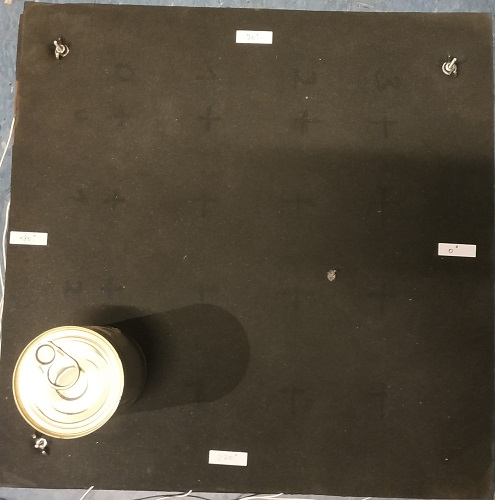
\includegraphics[width=0.75\linewidth]{img/badanie0_1.jpg} 
    \caption{Test 1} 
    % \vspace{4ex}
  \end{subfigure}%% 
  \begin{subfigure}[b]{0.5\linewidth}
    \centering
    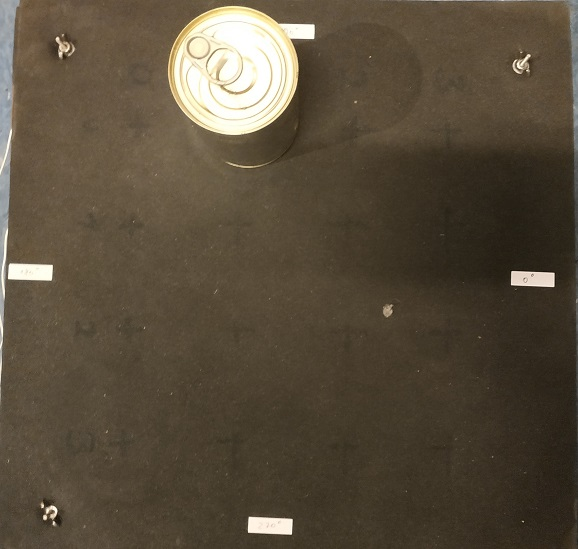
\includegraphics[width=0.75\linewidth]{img/badanie0_2.jpg}
    \caption{Test 2} 
    % \vspace{4ex}
  \end{subfigure} 
  
  \begin{subfigure}[b]{0.5\linewidth}
    \centering
    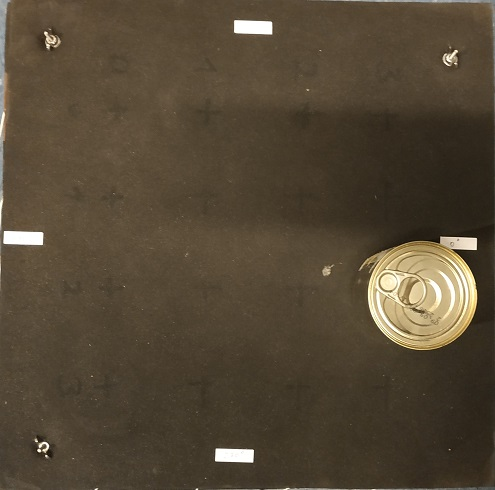
\includegraphics[width=0.75\linewidth]{img/badanie0_3.jpg} 
    \caption{Test 3}
  \end{subfigure}%%
  \begin{subfigure}[b]{0.5\linewidth}
    \centering
    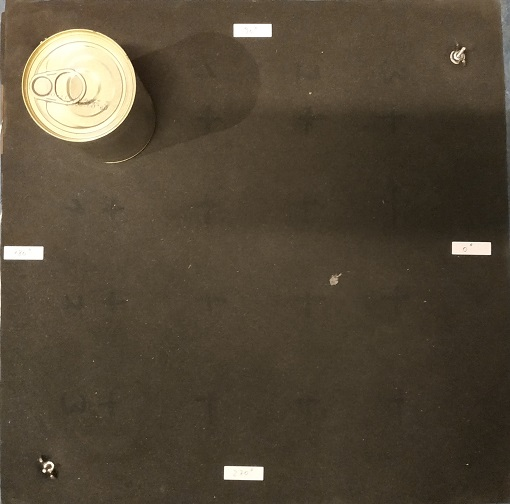
\includegraphics[width=0.75\linewidth]{img/badanie0_4.jpg}
    \caption{Test 4}
  \end{subfigure} 
  
  \begin{subfigure}[b]{0.5\linewidth}
    \centering
    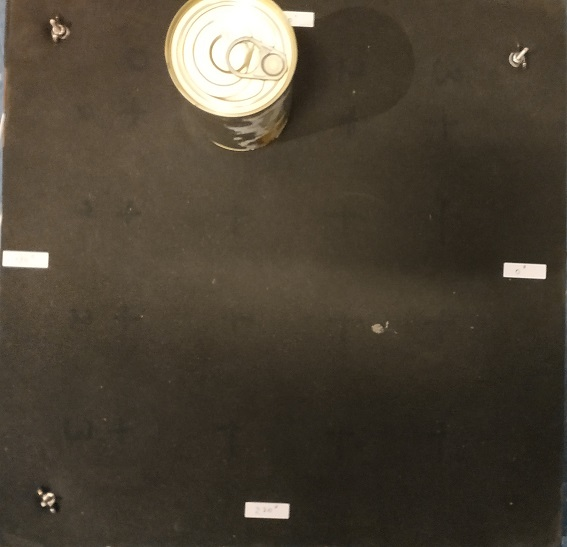
\includegraphics[width=0.75\linewidth]{img/badanie0_5.jpg}
    \caption{Test 5}
  \end{subfigure}%%
  \begin{subfigure}[b]{0.5\linewidth}
    \centering
    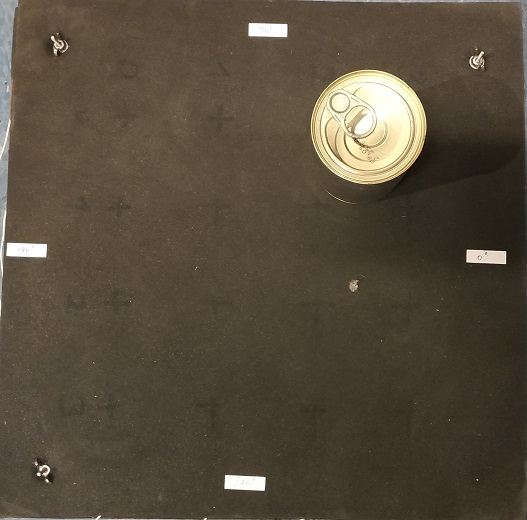
\includegraphics[width=0.75\linewidth]{img/badanie0_6.jpg}
    \caption{Test 6}
  \end{subfigure} 
  \centering
  \caption{Testy działania zaprogramowanego czujnika weryfikujące algorytm obliczający nacisk}
  \label{f_badanie0_pomiary} 
\end{figure}

\begin{table}[!h]
\centering
\caption{Wyniki testów algorytmu obliczającego nacisk}
\begin{tabular}{|l|r|r|}
\hline
Test   & \multicolumn{1}{l|}{Kąt} & \multicolumn{1}{l|}{Siła} \\ \hline
Brak obciążenia   & 45-50°                   & 40                        \\ \hline
Test 1 & 221°                     & 300                       \\ \hline
Test 2 & 100°                     & 500                       \\ \hline
Test 3 & 347°                     & 730                       \\ \hline
Test 4 & 134°                     & 670                       \\ \hline
Test 5 & 104°                     & 420                       \\ \hline
Test 6 & 45°                      & 700                       \\ \hline
\end{tabular}
\label{t_badanie0_wyniki}
\end{table}

Pierwszy pomiar zawiera wynik zwracany przez sterownik w momencie, kiedy prototyp nie był obciążony żadnym przedmiotem. Jak możemy zauważyć występuje tam szum, którego wartości cały czas nieznacznie się wahały. Otrzymywany szum nie osiągał dużych wartości i mógł zostać pominięty.

Kolejne pomiary wykonane z obciążeniem okazały się bardzo dobrze odwzorowywać miejsce przykładanej siły, nawet z obciążeniem znajdującym się pomiędzy polami czujnika. Z kolei w przypadku określania wartości przykładanej siły nacisku wyniki wydają się być niejednoznaczne. Otrzymywana wartość siły nacisku oscylowała podczas testów (również niezawartych w pracy) w granicach $300 - 750 g$ podczas, gdy prawdziwa waga obciążenia wynosiła $454 g$. Otrzymane w ten sposób wyniki posiadają bardzo złą dokładność względną pomiaru wynoszącą $-34\%/+65\%$. Mimo tak dużych rozbieżności pokazuje to pewną zależność, a same wyniki oscylują wokół faktycznej wagi i bardzo dobrze oddają kąt przyłożonej siły.

W celu znalezienia przyczyny tych rozbieżności wykonane zostało kilka niestandardowych pomiarów, gdzie to samo obciążenie ($454g$) było ustawione na krawędzi puszki czyniąc obszar nacisku dużo bardziej punktowym. W kolejnych testach zmieniany był punkt na prototypie, na którym spoczywało obciążenie. W ten sposób pomiary zostały wykonane zarówno idealnie na polu pomiarowym, jak i pomiędzy polami. Jak się okazało punkt przyłożenia obciążenia miał kluczowe znaczenie na otrzymywany wynik. Przy ułożeniu puszki na brzegu, bezpośrednio nad polem otrzymywane wyniki pomiarów były rzędu $\sim1100g$, a pomiędzy polami spadały one nawet do wartości $\sim200g$. Z otrzymanych danych jasno wynika, że miejsce przyłożenia nacisku ma duże znaczenie na odczytany pomiar i z tego powodu wykonane wcześniej pomiary posiadają tak duży rozrzut wartości zmierzonej masy. Może to świadczyć o tym, że materiał nośny niezbyt dobrze radzi sobie z rozkładaniem przyłożonej siły na boki, zamiast tego przenosi ją w~głąb, jednocześnie się uginając. Dodatkowo folia Velostat z racji, iż jest czujnikiem rezystancyjnym pokazuje dużo wyższe wyniki pomiarów w przypadku przyłożenia siły w jednym punkcie, niż~w~przypadku przyłożenia tej samej siły na większej powierzchni, nawet kiedy rozkłada się ona w całości na polu czujnika. Dodatkowe czynniki wpływające na wynik pomiaru zostały wykryte i~szczegółowo opisane w dalszych testach opisanych w dalszej części pracy.


% \subsubsection{Komunikacja przez USB}
\subsection{Warstwa komunikacyjna}
\label{ss_budowa_kom}

Komunikacja sterownika z komputerem nadrzędnym jest częścią, która stanowi o~użyteczności modułu sztucznej skóry. Jej rola polega na ciągłym i stabilnym wysyłaniu odbieranych informacji o otoczeniu do komputera sterującego całym robotem. Bez tej funkcji nawet poprawnie działająca sztuczna skóra nie ma żadnej wartości w systemie robota, ponieważ sam robot nie żadnych informacji o tym, że czujnik skóry cokolwiek wykrył.

Zastosowany w ramach pracy sposób komunikacji powinien być opisany powszechnie znanymi i rozpowszechnionymi standardami. Takie podejście pozwala na wybranie gotowych rozwiązań i na nietworzenie własnych, nie zawsze sprawdzonych rozwiązań. W~tym celu wybrane zostało jedno z najpopularniejszych obecnie rozwiązań - USB w standardzie 2.0. Gniazda w tym standardzie znajdują się obecnie w większości komputerów, również w urządzeniu, do którego sterownik będzie bezpośrednio dołączany. Standard ten wprowadzony już w 2000 roku oferuje prędkość przesyłu danych do 480Mbs, co jest w~pełni wystarczające dla obsługi sztucznej skóry. Wraz z samą komunikacją standard USB zapewnia zasilanie 5V dostarczane przez komputer. Pozwoliło to zasilić sterownik tym samym przewodem, po którym poprowadzona była komunikacja. Standard specyfikuje także przewody i gniazda, które można bez problemu nabyć na rynku \cite{b_manual_USB}.

Wykorzystanie do komunikacji standardu USB zmusiło mnie do wykonania projektu, który spełnia jego standardy. Nie zostały wybrane jednak mikrokontrolery STM z przeznaczonym do tego peryferium. Powodem takiej decyzji był chwilowy brak dostępności mikrokontrolerów o szukanych parametrach w tak małej (64 piny) obudowie układu scalonego. Problematyczna okazywała się także kwestia konieczności doinstalowania odpowiednich sterowników na komputerze do obsługi tak wykonanego układu. Dlatego ostatecznie do~komunikacji USB został wykorzystany dedykowany do tego układ CP2102 od Silicon Labs, który został zintegrowany na płytce drukowanej. Układ ten jest zgodny ze standardem USB 2.0 i pozwala na komunikację z prędkością do 12Mbs, co dla opracowywanego zastosowania jest wystarczające. Układ CP2102 jest konwerterem USB-UART co oznacza, że do poprawnej komunikacji mikrokontroler musi używać standardu UART. Standard UART jest dużo mniej skomplikowany niż wspomniany wcześniej USB, prostszy w obsłudze i~programowaniu. Konfiguracja wykorzystanego portu UART prezentowała się następująco: szybkość transmisji - 115200, liczba bitów - 8, bit parzystości - brak, bit stopu - 1. Układ CP2102 do poprawnej pracy wymaga również zainstalowania odpowiednich sterowników dostępnych na stronie producenta. Sterowniki te są również automatycznie instalowane wraz z systemem Linux Ubuntu \cite{b_site_CP2102}, na którym działał komputer nadrzędny.
% mikrokontroler

Aktualny projekt części elektronicznej zakłada również możliwość rozbudowy o dodatkowe sposoby komunikacji z komputerem nadrzędnym. Posiada wyprowadzone dodatkowe złącze, które może posłużyć właśnie do tego celu. Złącze to jest przystosowane bezpośrednio do~podłączenia tam popularnego modułu Bluetooth HC-05 \cite{b_site_HC-05_sklep}. Umożliwia to w przyszłości wykorzystanie urządzenia w systemach bezprzewodowych, czy też rozwiązaniach IOT.

Po ustaleniu wykorzystywanych fizycznie elementów ustalony został także standard przesyłanych informacji. W tym przypadku nie zostało wykorzystane żadne z istniejących i ustandaryzowanych rozwiązań. Standardy dostępne na rynku wymagają większych mocy obliczeniowych i czasowych do poprawnej pracy, w szczególności do obsługi błędów.
Dlatego zaimplementowane zostało dużo prostsze rozwiązanie, które w przeciwieństwie do standardów nie posiada tak dobrych zabezpieczeń. Wykorzystanie własnej implementacji zapewnia natomiast prostotę rozwiązania i niewielki nakład energii potrzebny do~przesłania danych.

Ramki przesyłające informacje są różne, w zależności od kierunku przesyłu danych. Ramka przesyłana do sterownika posiada lepszy opis i dokładny format ramek, aby nie zmienić konfiguracji sterownika przypadkowo. Ogólny wygląd przesyłanej ramki został przedstawiony w tabeli \ref{t_ramka_ogolna}, a dokładna zawartość przesyłanych danych w zależności od~funkcji w tabeli \ref{t_ramka_funkcja}. Ramki zaprojektowane w ten sposób zapewniają kilka podstawowych zabezpieczeń. Posiadane zabezpieczenia obejmują: pasywne zabezpieczenie przeciw przerwanym wiadomościom, zbyt długi czas przesyłu danych i możliwym zakłóceniom połączenia.

\begin{table}[!h]
\centering
\caption{Ramka danych przesyłanych przez USB do sterownika}
\begin{tabular}{|l|l|l|l|l|}
\hline
            & \multicolumn{1}{|c|}{Prefiks} & \multicolumn{1}{|c|}{Funkcja}                 & \multicolumn{1}{|c|}{Przesyłane dane}    & \multicolumn{1}{|c|}{Sufiks} \\ \hline
Liczba bajtów & 1      & 1                       & 7                  & 1      \\ \hline
Zawartość   & 0x02   & Typ przesyłanych danych & Dane do przesłania & 0x03   \\ \hline
\end{tabular}
\label{t_ramka_ogolna}
\end{table}

\begin{table}[!h]
\small
\centering
\caption{Tabela funkcji dostępnych w ramkach przesyłanych do sterownika}
\begin{tabular}{|l|l|c|l|l|l|l|l|l|}
\hline
\multicolumn{1}{|c|}{Funkcja} &
  \multicolumn{1}{c|}{\begin{tabular}[c]{@{}c@{}}Kod \\ funkcji\end{tabular}} &
  \multicolumn{7}{c|}{Dane} \\ \hline
\begin{tabular}[c]{@{}l@{}}Wyczyszczenie \\ pamięci\end{tabular} &
  0x01 &
  \multicolumn{7}{c|}{Bez znaczenia} \\ \hline
\begin{tabular}[c]{@{}l@{}}Potwierdzenie \\ wysłanych danych\end{tabular} &
  0x02 &
  \multicolumn{7}{c|}{Bez znaczenia} \\ \hline
\begin{tabular}[c]{@{}l@{}}Programowanie \\ pola czujnika \\ dotykowego\end{tabular} &
  0x10 &
  \multicolumn{1}{l|}{\begin{tabular}[c]{@{}l@{}}Pozostała\\ liczba pól\\ (1 bajt)\end{tabular}} &
  \begin{tabular}[c]{@{}l@{}}Klucz\\ (1 bajt)\end{tabular} &
  \begin{tabular}[c]{@{}l@{}}Kanał\\ (1 bajt)\end{tabular} &
  \multicolumn{2}{l|}{\begin{tabular}[c]{@{}l@{}}Kąt \\ (2 bajty)\end{tabular}} &
  \multicolumn{2}{l|}{\begin{tabular}[c]{@{}l@{}}Odległość \\ (2 bajty)\end{tabular}} \\ \hline
\end{tabular}
\label{t_ramka_funkcja}
\end{table}

Dane przesyłane do sterownika muszą zaczynać się od prefiksu, a kończyć sufiksem. Są one konieczne, aby sterownik mógł poprawnie otrzymać i zinterpretować przesyłane dane. Wewnątrz znajdują się przesyłane funkcje, których jest niewiele, ale wystarczają do~poprawnego działania sterownika. Funkcja czyszczenia pamięci jest konieczna, aby~poprawnie zaprogramować sterownik - wykonuje ona resetowanie pamięci Flash mikrokontrolera. Potwierdzenie wysłanych danych jest funkcją wysyłaną jako ostatnia, jako potwierdzenie zakończenia transmisji danych. Wysłanie tej funkcji pozwala na przejście programu mikrokontrolera do normalnej pętli pracy i wysyłanie pomiarów z czujnika do komputera. Niewysłanie tej funkcji wymaga zrestartowania mikrokontrolera, w~celu umożliwienia mu wysyłania danych do komputera.

Ostatnią i najważniejszą funkcją jest wysyłanie sterownikowi konfiguracji czujnika. Kod funkcji oznacza typ pola (w tym momencie jest jeden, ale w przyszłości można zaimplementować więcej). Po nim wysyłana jest liczba pól danego typu, które jeszcze zostaną przesłane. Ta informacja zapewnia spójność wysyłanych danych i zapobiega nieoczekiwanemu przerwaniu transmisji. Kolejno przesyłane są współrzędne pola (klucz i~kanał), jego wartość kąta wychylenia w~osi~$z$~robota oraz odległość czujnika od~środka robota.

Ramki przesyłane ze sterownika do komputera miały całkowicie inny kształt. Były one przeznaczone do bezpośredniego wyświetlania wysyłanych wartości na konsoli komunikacyjnej (w moim przypadku w programie PuTTY). Przesyłane liczby są wysyłane jako znaki zakodowane kodem ASCII, co wynika z konieczności ich bezpośredniego wyświetlania. Wysyłane przez sterownik ramki są przedstawione w tabeli \ref{t_ramka_przychodzi}. Wysyłanie wiadomości w~ten sposób wymagało dodatkowych przekształceń po obu komunikujących się stronach. Zmniejszyło to też wymiar przesyłanych danych do wartości 4-liczbowych. Takie podejście, mimo większej ilości zużywanych zasobów po obu stronach, pozwala na dużo szybszą i wygodniejszą współpracę ze sterownikiem, a także możliwość wykrywania błędów na~konsoli dowolnego komputera.

\begin{table}[!h]
\footnotesize
\centering
\caption{Ramka danych wysyłanych przez USB przez sterownik}
\begin{tabular}{|l|l|l|l|l|}
\hline
Wartość obliczonego kąta &
  , &
  Wartość obliczonej siły &
  ; &
  Przejście do następnej linii \\ \hline
\multicolumn{1}{|c|}{\begin{tabular}[c]{@{}c@{}}4 bajty - cyfry \\ kodowane ASCII\end{tabular}} &
  \multicolumn{1}{c|}{0x2C} &
  \multicolumn{1}{c|}{\begin{tabular}[c]{@{}c@{}}4 bajty - cyfry \\ kodowane ASCII\end{tabular}} &
  \multicolumn{1}{c|}{0x3B} &
  \multicolumn{1}{c|}{\begin{tabular}[c]{@{}c@{}}0x0D0A - znak powrotu\\ karetki i nowej linii\end{tabular}} \\ \hline
\end{tabular}
\label{t_ramka_przychodzi}
\end{table}

Ramka przesyłana przez sterownik do komputera, jak widać w tabeli \ref{t_ramka_przychodzi}, jest dużo prostsza i~ma tylko jedną konfigurację wypełnianą odpowiednimi danymi. Pierwsza część zawiera wartość obliczonego przez algorytm kąta siły, później dla czytelności i~oddzielenia danych wysyłany jest przecinek. Kolejną wysyłaną informacją jest wartość samej siły nacisku. Na koniec wysyłane są średnik oraz sekwencja znaków przenosząca karetkę (wskaźnik pisania na konsoli) na początek następnej linii konsoli.
